\documentclass[a4j,12pt]{jarticle}
\usepackage[dvipdfmx]{graphicx}
\usepackage[dvipdfmx]{hyperref}
%
% ---- 本文中でプログラムを掲載する際にキャプションを「リスト1」のようにする設定
%
% http://en.wikibooks.org/wiki/LaTeX/Floats,_Figures_and_Captions#Custom_floats
% 本文中でリストと表現されているところは
%
% \begin{program}..\end{program}を使います。
%
%  \begin{program}\centering
%  \begin{verbatim}
%
%  #define COM1_PORT (0x3f8)
%  #define COM1_LSR (COM1_PORT + 0)
%  #define COM1_RBR (COM1_PORT + 5)
%  unsigned char read_reg_byte(unsigned short port) {
%    unsigned char val;
%    asm volatile("inb %1, %0" : "=a"(val) : "Nd"(port));
%    return val;
%  }
%  \end{verbatim}
%  \caption{I/O マップド I/O での read\_reg\_byte() 関数およびレジスタの宣言}
%  \end{program}
%
% TODO: programをリストに変更する
%
\usepackage{float}
% 例では次のようになっているが...
%\newfloat{program}{thp}{lop}
\newfloat{program}{thp}{lop}
% ------------------------------------------------------------------------------

\title{第 5 回 I/O 仮想化「割り込み編・その 2 」}
\author{Takuya ASADA syuu@dokukino.com}
\begin{document}
\maketitle


\section{はじめに}

 前回の記事では、割り込み仮想化の話の前提とな
るx86アーキテクチャにおける割り込みのしくみを
各コンポーネントごとに解説しました(図1)。仮想
環境でどのように割り込みを実現するのか、前回解
説した各機能ごとに見ていきます。


\begin{figure}\centering
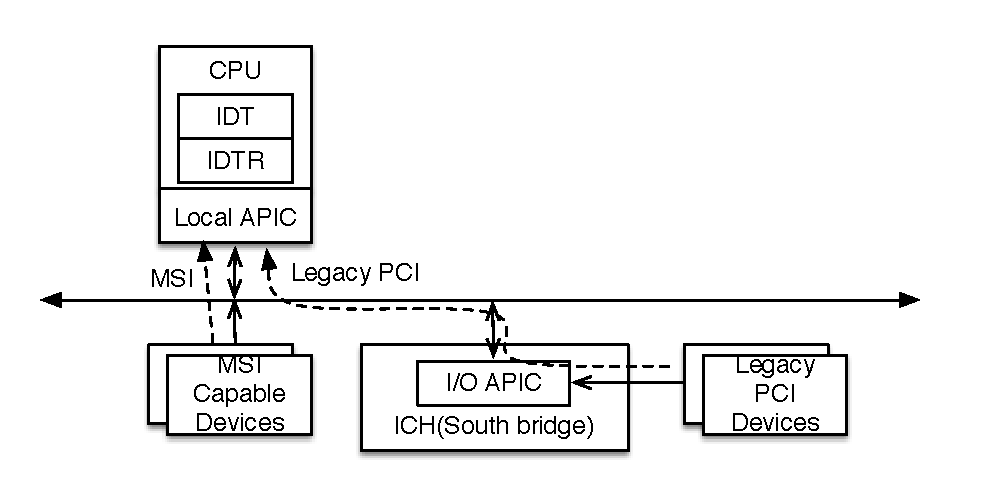
\includegraphics{figures/part5_fig1_interrupt_components.eps}
\caption{割り込みにかかわるコンポーネントと仮想化範囲}
\label{fig1}
\end{figure}


\section{仮想化における内部割り込みと外部割り込み}

 VT-x環境においては、内部割り込みはCPUがす
べて処理を行うため、基本的にハイパーバイザが介
入する必要がありません。一方、外部割り込みにつ
いては、ハイパーバイザの介入が必要となります。
それぞれを見ていきましょう。

\subsection*{CPU への割り込みの挿入}

 仮想 CPU で任意の割り込みを発生させるに
は、VMCS の VM-Entry Control Fields にある
VM-entry interruption-information field にベクタ
番号と割り込みタイプを書き込みます(表 1)。た
だし、このフィールドに値をセットして外部割り
込みを発生させるだけでは、Local APIC のレジ
スタ値は適切に更新されず、ハイパーバイザが新
しい値を計算しセットする必要があります。


\begin{table}\centering
\begin{tabular}{|p{4.5cm}|p{10cm}|} \hline

ビットポジション & 内容 \\
\hline
7:00             & ベクタ番号 \\
\hline
10:08            & 割り込みタイプ 通常は0 (外部割り込み) を使用 \\
\hline
11               & スタックに例外のerror codeをpush \\
\hline
31               & 有効化ビット \\
\hline
\end{tabular}
\caption{VM-entry interruption-information field}
\label{tab1}
\end{table}

\subsection*{内部割り込みの仮想化}

 実機での内部割り込みは、次の手順で処理されます。

\begin{enumerate}

\item ゲストマシン上のソフトウェアが例外を発生させるか、INT命令の実行によりCPUで内部割り込みが発生
\item CPUはIDT上のゲートデスクリプタを読み込み、割り込みハンドラを実行
\item 割り込みハンドラが内部割り込みを処理
\item IRET命令で直前のコンテキストへ復帰
\end{enumerate}

 これらはすべて、ハイパーバイザの介入が不要で
す2\verb|~|4については、 IDT/IDTR の仮想化にて説明し
ます。ただし、ここでもVMCSの設定により、内部
割り込みを契機としてVMExitを発生させることが
できます
  \footnote{
  VMCS の VM-Execution Control Fields の Exception Bitmap
  の各ビットが各例外のベクタ番号に対応していて、ここに1
  を設定するとその例外が発生した時に VMExit が発生するよう
  になります。通常の例外は基本的に VMExit する必要がありま
  せんが、連載第 2 回( Intel VT-x の概要とメモリ仮想化)で解説
  したシャドーページングを行うには、ページフォルト例外で
  のVMExit が必須になります。
  }

ただし、この利用方法は一般的ではありません。

\subsection*{外部割り込みの仮想化}

 内部割り込みはソフトウェアを起因としCPU内部
で発生するため、VT-xによりハイパーバイザの介入
なしに仮想化することが可能でした。一方、外部割
り込みは、ハイパーバイザが割り込みを送り込みま
す。これは、デバイスがソフトウェア的に、ハイ
パーバイザ内に実装されているためです。

\subsubsection*{I/O APIC を通して割り込む場合}
 実機でのI/O APICを通して割り込む場合の外部
割り込みは、次のような手順で処理されます。

\begin{enumerate}

\item デバイスが割り込みラインからI/O APICへ割り込みを送信
\item I/O APICが割り込みを受け取り、RedirectionTable Entryに指定されたDestination IDが示すLocal APICへ割り込みを転送
\item Local APICがCPUへ割り込み
\item CPUはIDT上のゲートデスクリプタをロードし、割り込みハンドラを実行
\item 割り込みハンドラが外部割り込みを処理
\item 割り込みハンドラがLocal APICへEOIを書き込み、割り込み処理の終了を伝達
\item IRET命令で直前のコンテキストへ復帰
\end{enumerate}


 このうち、4、5、7については内部割り込みと
同様の処理であり、ハイパーバイザの介入は必要あ
りません。1\verb|~|3は次のように仮想化されます。ま
ずあらかじめ、ゲストOSが割り込みを初期化する
ときにI/O APICのRedirection Table Entryへ宛先
Local APICが設定されます。実際にデバイスが使わ
れ始め、ハイパーバイザがデバイスのエミュレー
ションを行うと、割り込みを仮想CPUへ送る必要が
出てきます。
 デバイスエミュレータからの割り込みを受け、ハ
イパーバイザはデバイスに対応するRedirection
Table Entryの値を参照し、宛先の仮想CPUを選び
ます。宛先の仮想CPUが決定されたら、ハイパーバ
イザは宛先CPUのLocal APICのIRRレジスタを更
新し、VMCSに割り込みの挿入を設定します。割り
込み挿入が設定された仮想CPUがVMEnterされる
と、以降は内部割り込みと同様に、実機とほぼ同じ
手順で割り込みの受付が行われて割り込みハンドラ
が起動されます。
 6のEOI書き込みに関しては、Local APICのEOI
レジスタへのアクセスを、ハイパーバイザが介入し
てエミュレーションを行う必要があります。
 まとめると、外部割り込みを仮想化するには、ハイ
パーバイザでIO APIC・Local APICのエミュレーショ
ンを行い、仮想CPUへ割り込みを挿入する必要があ
ります。

\subsubsection*{MSI/MSI-X 割り込みを用いて割り込む場合}
 実機では、次の手順で処理されます。

\begin{enumerate}

\item デバイスがPCI Configuration Spaceに指定されたDestination IDが示すLocal APICへ割り込みを転送
\item Local APICがCPUへ割り込み
\item CPUはIDT上のゲートデスクリプタをロードし、割り込みハンドラを実行
\item 割り込みハンドラが外部割り込みを処理
\item 割り込みハンドラがLocal APICへEOIを書き込み、割り込み処理の終了を伝達
\item IRET命令で直前のコンテキストへ復帰
\end{enumerate}


 MSI/MSI-X割り込みを用いる場合の違いは、割
り込み先がI/O APICのRedirection Table Entryに
書いてあるのではなく、PCI Configuration Spaceに
書いてある、という点だけです。これを仮想化する
場合、ハイパーバイザで宛先の仮想CPUを選択する
ときの参照先が変わりますが、あとはI/O APICを
通じた割り込みと同じです。


\section{IDT/IDTR と割り込みハンドラ}

 IDT/IDTRや割り込みハンドラに関しては、とくに
ハイパーバイザが介入すべき処理はありません。この
ためVMExitは発生せず、すべてCPUが仮想化を行
います\footnote{
ただし、割り込みハンドラ内で IO ポートアクセスなどの操作
を行えば VMExit が発生する操作を行えば、そこでは VMExit
が発生します。 
}。
VT-x において一部の汎用レジスタはVMX
root mode/VMX non-root modeの切り替えときにコン
テキストをハイパーバイザで保存する必要がありまし
た。しかし、IDTRレジスタのコンテキスト保存/復
帰については、ハイパーバイザは関与しません。
 これは、CPUによって行われるためです。ゲスト
マシン上のIDTの作成や割り込みハンドラのアドレ
スの設定は、通常のメモリアクセアスと同様に行わ
れます。また、VT-x non-root mode では、実機での
動作と同様に割り込みや例外を受け付け、割り込み
ハンドラを実行する機能が備わっています。ゲスト
マシンのIDTRは、 IDTの構築後に設定されます。な
お、一般的な手法ではありませんが、VMCSの設
定\footnote{
VMCS の VM-Execution Control Fields の Secondary
Processor-Based VM-Execution Controls にある Descriptor-
table exiting にビットを立てることで、LGDT、LIDT、LLDT、
LTR、SGDT、SIDT、SLDT、STR の各命令を実行しようとした
時に VMExit するようになります。 
}
によりIDTRへの読み書きを契機としてVMExit
を発生させることもできます\footnote{
この場合、ハイパーバイザは ID のシャドーイングを行ってゲ
スト OS が意図する割り込みハンドラと異なる割り込みハンド
ラを設定できます。また、 IDTR へのアクセスをイベントとし
て受け取り、デバッグ機能を実装することもできます。
}。
 このうち、2\verb|~|4でハイパーバイザの介入が不要
であることは、すでに説明しました。1ですが、ゲ
スト環境から内部を発生させ、割り込みハンドラを
起動する処理の中で、とくにハイパーバイザの介入
は必要ありません。
 ただし、ここでもVMCSの設定により、内部割り
込みを契機としてVMExitを発生できま。この場合、
内部割り込みをゲストOSに渡さずハイパーバイザ
で横取りして処理をしたり、デバッグ機能としてゲ
スト環境上の内部割り込みの回数をカウントしたり
といった機能を実装できます。しかしながら、その
ような使い方は一般的ではありません。
 まとめると、内部割り込みの一連の処理に関して
は、特にハイパーバイザが介入すべき処理はありま
せん。このためVMExitは発生せず、すべてCPUが
仮想化を行います。



\section{Local APIC の仮想化}

 Local APICはメモリマップドI/Oでアクセスする
ため、通常のメモリマップドI/Oの仮想化手法が使
えます。しかし、高速化のためにVT-xにはLocal
APICへのアクセスを特別扱いしてハンドルする機
能が実装されています。このことは、連載第3回(I/
O仮想化「デバイスI/O編」)で解説しました。つま
り、図1で示したように、部分的にVT-xによる仮想
化支援を受けることができます。
 しかしながら、このVT-xによる仮想化支援機能
はハイパーバイザが何もしなくても完全にCPU側で
レジスタ値の更新などを行ってくれるというもので
はありません。 CPUへ外部割り込みを挿入する場合、
ゲストOSから見てつじつまが合わなくならないよ
うLocalAPICのレジスタ値を同時に設定する作業は
ハイパーバイザから行う必要があります。具体的に
は、次の操作を行います。形になります。実機での
外部割り込みは、次の手順で処理されます。

\begin{enumerate}

\item 割り込み発生時点でIRRレジスタに割り込むベクタ番号のビットをセット
\item 仮想CPUがVMExitするのを待つ/またはIPIなどを用いてVMExitさせる
\item IRRにセットされた最高優先度のビットをクリア、同じビットをISRにセット
\item TPRとISRの値に基いてPPRを更新
\item VM-entry interruption-information fieldに割り込みをセット
\item VMEnterして割り込みを発生させる

\end{enumerate}

 また、割り込みハンドラの終了を通知するために
ゲストOSがEOIレジスタへ書き込んできたときに
も、ハイパーバイザの介入が必要です。具体的には、
次の作業を行います。

\begin{enumerate}

\item EOIへの書き込みによりVMExit
\item IRRが0ならVMEnterしてゲストへ復帰?IRRに値があればIRRにセットされた最高優先度のビットをクリア、同じビットをISRにセット
\item TPRとISRの値に基いてPPRを更新
\item VM-entry interruption-information fieldに割り込みをセット
\item VMEnterして割り込みを発生させる
\end{enumerate}

 こちらも、前回の記事で解説した実機上のLocal
APICの挙動と同じです。


\section{I/O APIC の仮想化}

 I/O APICもゲストOSからメモリマップドI/Oで
アクセスされます。ただし、Local APICと異なり高
速化用の特別なVMExitなどの仮想化支援機能はあ
りません。使われ方としては、前述のとおりゲスト
OSの初期化時に割り込み先CPUの設定をメモリ
マップドI/O経由で受け取り、仮想デバイスから割
り込みを送るときの仮想CPU選択に設定された値を
用います。


\section{MSI/MSI-X 割り込みの仮想化}

 MSI/MSI-X割り込みの場合は、PCI Configuration
Spaceへの書き込みにより割り込み先CPUの設定を
受け取ります。書き込むデバイスやレジスタの
フォーマットは違いますが 、使い方はほぼI/O
APICと変わりません。\footnote{
参考資料(\href{http://d.hatena.ne.jp/syuu1228/20120105/1325757315}{http://d.hatena.ne.jp/syuu1228/20120105/1325757315})
}   


\section{物理ハードウェアからの割り込みへの対処}

 VMX non-root modeの実行中に物理ハードウェア
から割り込みが来た場合、ハイパーバイザでこれを
受け取り割り込みハンドラを起動して処理する必要
があります。このために、ハイパーバイザはVMCS
の初期化時にVM-Execution Control FieldsのPin-
Based VM-Execution ControlsにあるExternal-
interrupt exitingにビットをセットします。これによ
り、ゲストマシンは外部割り込み発生時にVMExit
するようになります。また、VM-Exit Control Fieldsに
あるVM-Exit ControlsのAcknowledge interrupt on
exitビットを1に設定した場合、外部割り込みは
VMExit時に"acknowledged"になり、割り込みベク
タ番号はVM-Exit information fieldsのVM-exit
interruption informationに保存されます。VMMはこ
のベクタ番号を参照して、割り込みハンドラを起動
し割り込みを処理します。
 一方、Acknowledge interrupt on exitビットを0に
設定した場合は割り込みは"acknowledge"されず、
RFLAGSレジスタのIFビットでマスクされている
状態になります。このままIFフラグをセットすれ
ば、 IDTに設定された割り込みハンドラが起動して割
り込みを処理できます。通常のOSの上にハイパー
バイザを実装する方式では、 IDTによる割り込みハン
ドルが行われているため、後者の方法を取る場合が
ほとんどです。


\section{まとめ}

 いかがでしたでしょうか。今回は Intel VT-x にお
ける割り込みの仮想化方法を中心に解説してきまし
た。次回はソフトウェア側の実装に移り、「VT-xを
用いたハイパーバイザの実装方法の基礎」を中心に解
説します。
\section{ライセンス}
Copyright (c) 2014 Takuya ASADA.
全ての原稿データ は クリエイティブ・コモンズ 表示 - 継承 4.0 国際 ライセンスの下に提供されています。


\end{document}
